In diesem Kapitel soll der experimentelle Aufbau des gesamten Lasersystems und
dessen Kopplung an die Vakuumapperatur und den Quadrupol beschrieben werden.
Zunächst wird ein Überblick über das gesamte System gegeben (Abschn.
\ref{sec:gesamtaufbau}). Abschnitt \ref{sec:lasersystem} beschriebt den gesamten
optischen Aufbau inklusive Laserstabilisierung. Die Weiterverarbeitung der
Laserinformation und die Stabilisierung sollen in Abschn.
\ref{sec:elektronik_laserkontrolle} genauer betrachtet werden. Da
hard- und softwareseitige Implementierung der Laserkontrolle eng miteinander verknüpft
sind, kommt es zu Überschneidungen mit Kap. \ref{kap:software}, in dem die
softwareseitige Realisierung genau erklärt wird. In Abschn.
\ref{sec:vakuum-aparatur_qms} wird kurz speziell auf die verwendete
Vakuumaparatur und dem daran gekoppelten Quadrupolmassenseperator eingegangen.

\section{Gesamtaufbau}\label{sec:gesamtaufbau}
\begin{figure}[h]
 	\centering
 	\fbox{\parbox{\dimexpr \linewidth - 2\fboxrule - 2\fboxsep}{
 	\centering
	    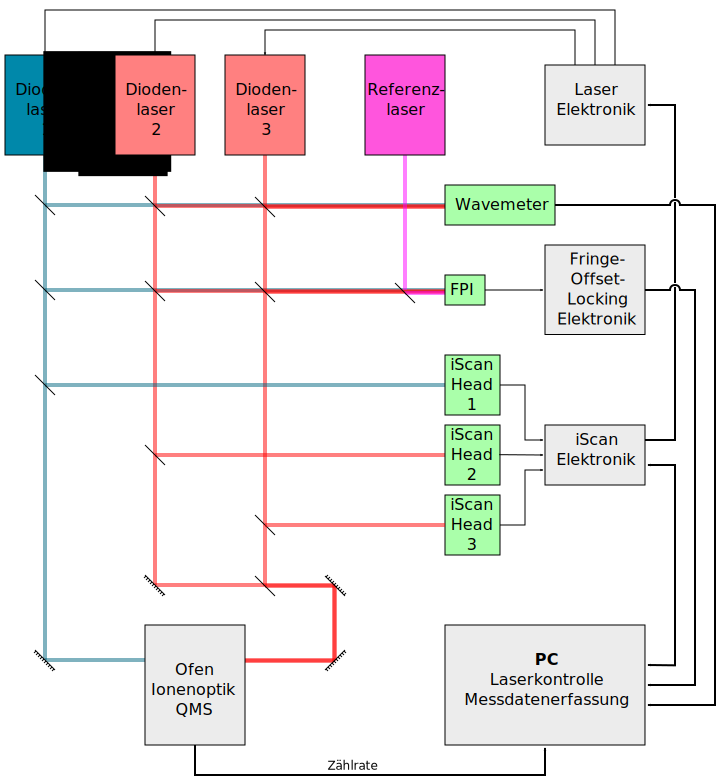
\includegraphics[width=\textwidth-2cm]{gfx/experimenteller_aufbau_gesamt}
	}}
	\caption[Gesamter experimenteller Aufbau, schematisch]{Gesamter experimenteller
	Aufbau des Systems (schematisch).}\label{fig:experimenteller_aufbau_gesamt}
\end{figure}
Abbildung \ref{fig:experimenteller_aufbau_gesamt} zeigt schematisch den gesamten
Aufbau des Systems. Das zur resonanten Anregung nötige Licht wird mit drei
Diodenlaser erzeugt. Der größte Teil des Lichts wird möglichst
direkt in die Vakuumaparatur, die aus einem Ofen für das Ausheizen der Atome,
einer Ionenoptik für die Kontrolle der erzeugten Ionen und einem
Quadrupolmassenseperator (QMS) zur Massenselktion der Ionen besteht, geführt.
Die Einstrahlung der Laser erfolgt aus den in Abschn. \ref{sec:linienprofil}
erleuterten Gründen transversal zum aus dem Ofen austretenden kollimierten Atomstrahl.
Abgriffe der Hauptstrahlen führen das Laserlicht eines jeden Lasers in ein
Wavemeter, das die Absolutwellenlängen liefert und an einen PC weiterleitet.
Zwei jeweils weitere Abgriffe führen die Strahlen in die Optiken iScan Heads und FPI der zwei verwendeten
Laserstabilisierungen. Die dort erzeugten Signale werden an die jeweilige Elektronik
weitergeleitet. Die Elektronik eines iScan Heads ist die iScans control units, die direkt an die Elektronik des entsprechenden Laser
angeschlossen ist und sowohl die Spannung des Laserpiezos als auch den Strom
der Laserdiode moduliert. Die Elektronik des Fringe-Offset-Locking bereitet die
analogen Signale des FPIs digital auf und leitet sie weiter an den PC, der
gleichzeitig mit den iScan control units bidirektional verbunden ist und die
Regelung der iScan-Sollwerte übernimmt. Weiterhin kann mit dem PC die Zählrate
der Ionen, die einzeln durch ein hinter dem QMS angebrachten Channeltron
detektiert werden, aufgenommen werden. Die Steuerung des Massenseperators
bezüglich der Einstellung bzw. des Scans bestimmter Massen durch den PC wurde im
Rahmen dieser Arbeit noch nicht realisiert, soll aber nachträglich implementiert
werden. Alternativ wird hierfür bis zum Abschluss dieser Arbeit noch ein PC des
Vorgängersystems verwendet.

\section{Lasersystem}\label{sec:lasersystem}
\begin{figure}[h]
 	\centering
 	\fbox{\parbox{\dimexpr \linewidth - 2\fboxrule - 2\fboxsep}{
 	\centering
	    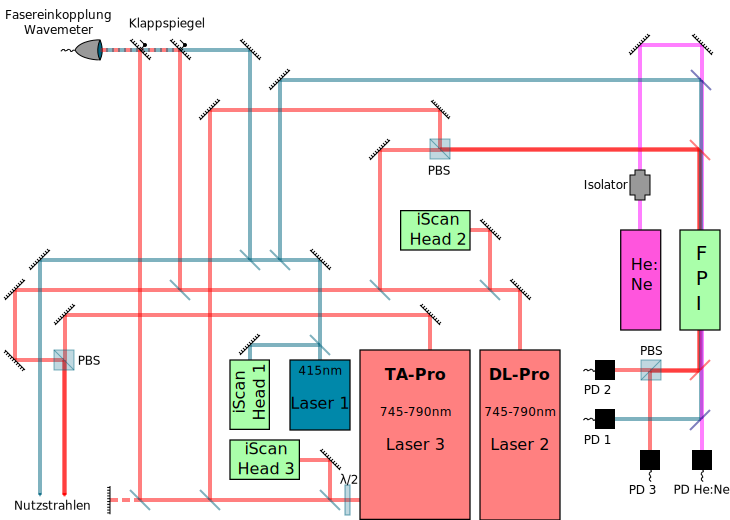
\includegraphics[width=\textwidth-2cm]{gfx/experimenteller_aufbau_lasersystem}
	    }}
	\caption[Experimenteller Aufbau des Lasersystems, schematisch]{Experimenteller
	Aufbau des Lasersystems
	(schematisch).}\label{fig:experimenteller_aufbau_lasersystem}
\end{figure}
Ein detaillierter Aufbau des Lasersystems wird schematisch durch Abb.
\ref{fig:experimenteller_aufbau_lasersystem} veranschaulicht und ist als
Fotografie in Abb. \ref{fig:experimenteller_aufbau_lasersystem_foto} noch einmal
zu sehen.\par
Das Laserlicht für den ersten Anregungsschritt wird in einem nach dem
Littrow-Design gebauten Diodenlaser erzeugt. Eingebaut ist eine blaue
$415\,$nm-Laserdiode mit einem Verstärkungsprofil von $\pm1\,$nm bei
zugeschalteten externen Resonator. Der modensprungfreie Verstimmungsbereich ist
mit $15\,$GHz spezifiziert. In manchen Moden wurden allerdings auch Verstimmungsbereiche
von bis zu $20\,$GHz erreicht. Das Laserlicht des zweiten und dritten
Anregungsschritts wird mit zwei kommerziellen, ebenfalls im Littrow-Design
gebauten, roten Diodenlasern der Firma Toptica erzeugt.
Beide Dioden haben ein spezifiziertes Verstärkungsprofil von
$745\,$nm bis $790\,$nm und einen modensprungfreien Verstimmungsbereich von bis
zu $30\,$GHz, was bestätigt wurde. Weiterhin kann das Laserlicht der Diode für
den dritten Anregungsschritt mit einem Trapezverstärker wahlweise bis auf eine
Leistung von $1,5\,$W verstärkt werden. Neben dem leistungsstarken Nutzstrahl
gibt es noch die Möglichkeit, einen Teil des zum Injection-Seeding verwendeten
Masterlaserstrahl abzugreifen (links unten am TA-Pro in Abb.
\ref{fig:experimenteller_aufbau_lasersystem}). Für den ersten bzw.
zweiten Anregungsschritt können ca. $7\,$mW bzw. ca. $60\,$mW bei Diodenströmen von ca. $35\,$mA bzw. ca.
$120\,$mA erreicht werden, was für die Untersuchung von Uran-Isotopen
ausreichend ist. Die Sättigungsleistungen sind im ersten Schritt $<1\,$mW, im
zweiten Schritt wenige mW und im dritten Schritt wenige $100\,$mW. Tabelle \ref{tab:laser_spezifikationen} listet noch einmal alle
Laser-Spezifikationen auf.
***blabla*Referenz zu Lasermanuals / Diodenmanuals*blabla***\par
\begin{table}
	%Summe der Breiten muss 0.91 mal \textwidth sein.
	\begin{tabular}{p{0.23\textwidth}|p{0.24\textwidth}p{0.24\textwidth}p{0.24\textwidth}}
		\toprule
		& Laser 1 & Laser 2 & Laser 3\\
		\midrule[1px]
		\hline
		Bezeichnung & Eigenbau & DL-Pro & TA-Pro\\
		Wellenlänge & $415\pm1\,$nm & $745\,$-$790\,$nm & $745\,$-$790\,$nm\\
		max. Leistung & $7\,$mW & $60\,$mW & $1,5\,$W\\
		nötige Leistung & $<1\,$mW & $xx\,$mW & $xxx\,$mW\\
		Externer Resonator & Littrow & Littrow & Littrow\\
		\bottomrule[1px]
	\end{tabular}
	\caption[Spezifikationen der verwendeten Diodenlaser]{Spezifikationen der
	verwendeten Diodenlaser}
	\label{tab:laser_spezifikationen}
\end{table}
Die Teilstrahlen für die Stabilisierung der iScans werden auf Grund der in
\ref{subsec:iScan} erklärten Empfindlichkeit auf räumliche Drifts möglichst
direkt in die iScan Heads geführt, damit die Hebelwirkung bei Drifts möglichst
gering ist. Für das iScan für Laser 3 muss die Polarisation mit einem
$\nicefrac{\lambda}{2}$-Plättchen gedreht werden.\par Die Abgriffe für das Wavemeter des Typs ***blabla*Typ*blabla*** von der Firma
High Finesse müssen mit Klappspiegeln einzeln ausgewählt werden, da immer nur das
Licht eines Lasers im Wavemeter analysiert werden kann. Die Genauigkeit des
Wavemeters von $30\,$MHz hat ***blabla*Referenz zu Wavemeter-Manual*blabla***,
würde es zur Frequenzstabilisierung nicht genügen, ist aber für das Finden von Resonanzen und wie schon erwähnt zum Berechnen der Relativfrequenzen nach Gl. \eqref{eq:FPI_frequenzdrift_03}
ausreichend.\par
Für das Fringe-Offset-Locking muss das Licht aller drei zu stabilisierenden
Laser vor dem FPI zusammengeführt und danach wieder getrennt werden. Da die
Wellenlängen von Laser 2 und 3 sehr nahe beieinander liegen, muss das Licht
dieser Laser mit Polarisationsstrahlteiler zusammengeführt und getrennt werden.
Dabei ist zu beachten, dass die Verluste durch die jeweils falsche Polarisation
der Laser möglichst gering ist, was durch optionales Drehen der
Polarisation mit $\nicefrac{\lambda}{2}$-Plättchen möglich ist. Die Überlagerung
mit dem blauen Licht des ersten Lasers und dem He:Ne-Laser kann mit
dichroitischen Spiegeln realisiert werden. Diese sind dafür ausgelegt bestimmte
Wellenlängenbereiche zu reflektieren, während andere bestimmte Bereiche
transmittiert werden. Die Trennung der Strahlen erfolgt nach dem selben
Prinzip. Hinter dem gerampten FPI wird das Fringepattern aller vier Laser
getrennt mit Photodioden aufgenommen. Das FPI hat nach Angaben aus dem Jahre 199x einen
freien Spektralbereich von $298,xx\,$MHz. Im nah-infraroten Bereich hat es die
größte Finesse, wohingegen im blauen Bereich die Finesse sehr schlecht ist.
Das Fringe-Offset-Locking ist damit zwar noch möglich, es wird allerdings
angestrebt, ein anderes Interferomter zu verwenden. Dieses wird momentan
noch in dem parallel laufenden alten System verwendet, das während dem
Entstehen dieser Arbeit noch als Referenzsystem eingesetzt und in
\ref{sec:altes_lasersystem} kurz beschrieben wird.\par
Die Hauptstrahlen werden an ein Pereskop geführt, über das das Licht in einen
anderen Raum an die Vakuum-Aparatur transportiert wird, wobei das Licht von
Laser 2 und 3 wieder durch Polarisationstrennung überlagert ist. Der
Strahltransport über das Pereskop ist Teil einer Vorablösung, da auf dem
Lasertisch der Vakuum-Aparatur das alte Lasersystem aufgebaut ist.\par
Der He:Ne-Laser ist gegen Rückreflexe aus dem FPI durch einen optischen Isolator
geschützt. Ebenso hat der zweite Laser vor dem Masterlaserabgriff und nach dem
Trapezverstärker einen Isolator. Laser 1 und 2 haben momentan noch keinen
Isolator. Es soll jedoch in Zukunft jeweil ein Isolator zwischengeschaltet
werden.

\section{Elektronik der Laserkontrolle}\label{sec:elektronik_laserkontrolle} In
diesem Abschnitt wird die Verarbeitung der Signale zur Laserkontrolle schematisch erklärt. Für
Schaltpläne und interne elektronische Abläufe verschiedener Komponenten sei auf
den Anhang verwiesen. Abbildung \ref{fig:experimenteller_aufbau_elektronik_laserkontrolle} zeigt den
schematischen Aufbau der Elektronik für die Laserkontrolle.\par
\begin{figure}[h]
 	\centering
 	\fbox{\parbox{\dimexpr \linewidth - 2\fboxrule - 2\fboxsep}{
 	\centering
	    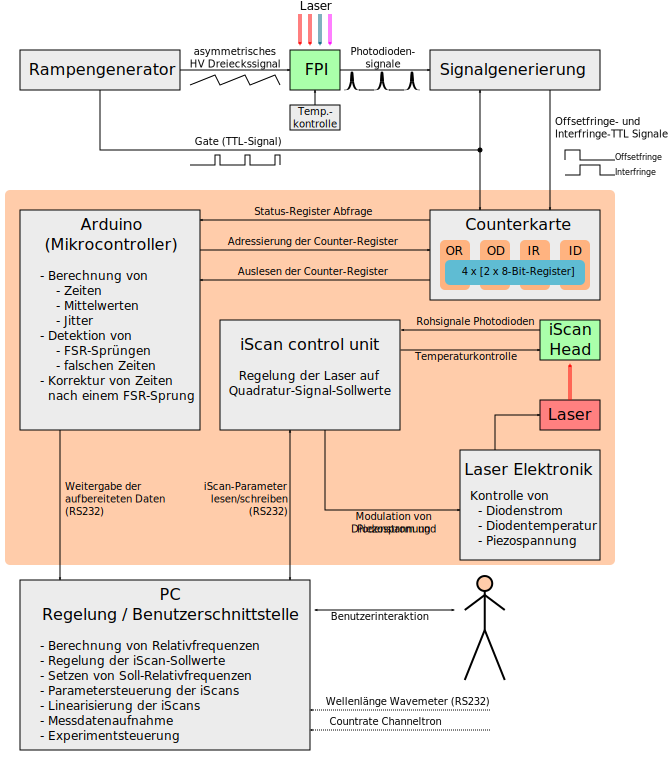
\includegraphics[width=\textwidth-2cm]{gfx/experimenteller_aufbau_elektronik_laserkontrolle}
	    }}
	\caption[Experimenteller Aufbau der Laserkontollelektronik,
	schematisch]{Experimenteller Aufbau der Elektronik der Laserkontrolle
	(schematisch).}\label{fig:experimenteller_aufbau_elektronik_laserkontrolle}
\end{figure}
Das FPI wird durch einen Rampengenerator in seiner Länge linear durchgefahren.
Dazu wird ein asymetrisches Dreieckssignal mit ca. $60\,$Hz erzeugt, welches die wie in Abb.
\ref{fig:FPI_signal-zeitverlauf}(b) gezeigte Fringepattern für jeden Laser
an den Photodioden hinter dem FPI erzeugt. Außerdem gibt der Rampengenerator
ein TTL-Signal aus, des bei fallender Spannungsflanke HIGH und bei
steigender Spannungsflanke LOW ist. Die fallende bzw. steigende Flanke dieses
\textit{Gates} signalisiert also den Start bzw. das Ende der Spannungsrampe
und wird als Triggersignal verwendet. Die Photodiodensignale und das
Gate werden an einen Signalgenerator weitergegeben, welcher über Ableiten der
Fringesignale die wie in \ref{fig:FPI_signal-zeitverlauf}(d,e) gezeigten TTL-Pulse erzeugt.
Wie dies genau geschieht wird in Anh. \ref{anh:kap:signalgenerierung}
beschrieben. Es ist weiterhin möglich, eine \textit{Delay} in der Detektion des
ersten Fringes einzustellen, damit Nichtlinearitäten zu Beginn der Rampe
ignoriert werden.\par
Der im Folgenden beschriebene Ablauf ist für jeden zu stabilisierenden Laser
gleich. Daher wird dieser Teil exemplarisch für einen Laser und den
Referenzlaser beschrieben. Die durch den Offsetfringe und Interfringe erzeugten
TTL-Pulse des sowohl zu stabilisierenden Lasers als auch des Referenzlasers,
sowie das Gate werden an eine Counterkarte weitergeleitet. Diese besteht aus
vier 16-Bit-Countern und einem Taktgeber mit einstellbarer Taktrate ($1,25\,$,
$2,5\,$, $5\,$ und $10\,$MHz), wodurch unterschiedliche Zeitauflösungen möglich
sind ($0,8\,$, $0,4\,$, $0,2\,$ und $0,1\,$\textmu s).
Wird das Gate auf LOW gesetzt (Beginn der steigenden Spannungsflanke), werden
alle Counter freigeschaltet. Wenn die durch
das Delay etwas verzögerten TTL-Signale der Offsetfringes auf HIGH gesetzt werden, beginnen die
entsprechenden Counter der Offsetfringes (OR und OD) zu zählen. Beim eintreten
der Interfringes werden die Counter gestoppt und die Counter für die
Interfringezeiten gestartet (IR und ID). Am Ende der steigenden Spannungsflanke
wird das Gate auf HIGH gesetzt und die Counter werden gesperrt. Beim Stoppen eines
jeden Counters liegen die Counterwerte in jeweils 2x8-Bit-Registern
(\textit{Upper Byte} und \textit{Lower Byte}) vor und es wird jeweils ein
\textit{Ready-Bit} gesetzt, welches Abrufbereitschaft der entsprechenden
Counterwerte signalisiert.\par
Die Ready-Bits sind über ein \textit{Statusregister} auslesbar. Die Adressierung
der einzelnen Counterregister wird über einen \textit{Adressbus} mit vier Bits
gesteuert, dessen Kodierung in Tab. \ref{tab:adressbus_kodierung} aufgeschlüsselt ist.
\begin{table}
	%Summe der Breiten muss 0.91 mal \textwidth sein.
	\begin{tabular}{p{0.1\textwidth}p{0.1\textwidth}p{0.1\textwidth}p{0.1\textwidth}|p{0.51\textwidth}}
		\toprule
		Enable & Addr. 1 & Addr. 2 & Addr. 3 & Wirkung\\
		\midrule[1px]
		\hline
		L & - & - & - & Adressierung deaktiviert\\
		H & L & L & L & Lower Byte Offsetfringe Referenzlaser\\
		H & L & L & H & Upper Byte Offsetfringe Referenzlaser\\
		H & L & H & L & Lower Byte Interfringe Referenzlaser\\
		H & L & H & H & Upper Byte Interfringe Referenzlaser\\
		H & H & L & L & Lower Byte Offsetfringe Diodenlaser\\
		H & H & L & H & Upper Byte Offsetfringe Diodenlaser\\
		H & H & H & L & Lower Byte Interfringe Diodenlaser\\
		H & H & H & H & Upper Byte Interfringe Diodenlaser\\
		\bottomrule[1px]
	\end{tabular}
	\caption[Adressierung Counterregister]{Aufschlüsselung der Adressierung der
	Counterregister}
	\label{tab:adressbus_kodierung}
\end{table}
Dabei sind \textit{Addr. 1} bis \textit{3} die Adressleitungen. Über
\textit{Enable} kann die Adressierung aktiviert und deaktiviert werden. Sehr
wichtig hierbei ist, dass einem Adressierungswechsel auf ein anderes
Counterregister die Adressierung immer deaktiviert werden muss. Andernfalls kann
es zur Zerstörung der Counter kommen.\par
Die Auslese und Weiterverarbeitung der Werte muss nun bis spätestens zur
nächsten steigenden Spannungsrampe abgeschlossen sein, damit die neuen
Rampensignale abgearbeitet werden können und es zu keinen Datenverlusten kommt.
Da bei einem PC mit Windows-Betriebssystem die Prozessverwaltung auf Grund von
unvorhersehbaren Interupts nie deterministisch ist, ist es sehr unsicher die
Daten direkt mit einem PC zu verarbeiten. Daher werden die Daten zunächst von
einem Mikrocontroller aufbereitet und anschließend an einen PC gesendet. Als
Mikrocontroller eignet sich dafür hervorragend die Entwicklungsplattform
\textit{Arduino$^\text{\textregistered}$}\footnote{http://www.arduino.cc}. Diese
wird verwendet, da sich das Projekt auch nach Abschluss dieser Arbeit noch in
der Entwicklungsphase befindet und der Arduino eine unkomplizierte Handhabung
und Programmierung bietet, was für Entwicklungszwecke gegenüber einem einfachen
Mikrocontroller-Chip sehr viel vorteilhafter ist. Der hier eingesetzte
\textit{Arduino Mega 2560} bietet 54 digitale Ein- und Ausgänge, hat eine
Taktrate von $16\,$MHz Flashspeicher von $256\,$kb für den binären Programmcode.
